\documentclass[twoside, a4paper]{article}
\usepackage{amsmath}
\usepackage{float}
\usepackage{graphicx}
\usepackage{url}
\newfloat{program}{thp}{lop}
\floatname{program}{Listing}
\author{Lukas Hofmaier}
\title{Type class laws}

\begin{document}
\maketitle
\tableofcontents

\section{Introduction}
\label{sec:intro}

Formal verification is a tool use for software application with the aim of providing a high reliability. The first formally verfified microkernel, seL4 was verified using Haskell. Haskell was used because programmers can reason about the source code \cite{Klein09}. Correctness is specified in form of equations. The source code must satisfy this equations. Programmers can use equational reasoning to verify the correctness of these equations.
Purely functional programming languages are easier to reason about as imperative or object-oriented languages.

\section{Type classes}
\label{sec:typeclasses}

A type class is like an interface. It defines behavior of a type. A type becomes an instance of a type class if it implements the functions of the type class. When a type class implements a type class, the type provides the functions, which the type class defines.
The concept of a type class is explained with the function \verb|show| from the \verb|Prelude|-Library. \verb|show| converts a given type into a character string.
\begin{verbatim}
show :: Show a => a -> String
\end{verbatim}
The \verb|Show a| before the \verb|=>| is a class constraint. \verb|a| is a type variable. The signature means that \verb|show| takes something that implements the type class \verb|Show| and returns a string. \verb|Show| is a type class. 
Any type that implements \verb|Show| can be converted to a character string. Types in this class are \verb|Bool|, \verb|Char|, \verb|Int|, \verb|Float|, \verb|Double| etc.

A type class is defined as follows: For example \verb|Show|:
\begin{verbatim}
class Show a where
    show :: a -> String
\end{verbatim}
The keyword \verb|class| defines a new type class. \verb|a| is the type variable. It can be replaced with the type that implements the type class.

Once we have a class we make types instances of that class. If we have a type \verb|Person| with an name and an email address:
\begin{verbatim}
data Person = Person { name :: String
                       email :: String
                     }
\end{verbatim}

To print out a person the type \verb|Person| has to be an instance of \verb|Show|.

\begin{verbatim}
instance Show Person where
    show (Person name _) = name
\end{verbatim}

There many other useful type classes in the standard library.

\begin{description}
\item[Ord] Types with an order relation implement \verb|Ord|.
\item[Eq] For types that can be equated.
\item[Read] Types that can be convertet from a string.
\end{description}

\subsection{Polymorphism and type classes}
\label{sec:polymorphism}

There are two types of polymorphism in Haskell \cite{Cardelli}.
\begin{description}
\item[Parametric polymorphism] Refers to a type that contains type variable. For example the type of the function \verb|id| is 
\begin{verbatim}
id:: a -> a
\end{verbatim}
The \verb|id| function can be used with any type. There are no constraints. At compile time the type variable are substituted with a concrete type. For example
\verb|Char -> Char|.
\item[Ad-hoc polymorphism] It's a synonym for function overloading or operator overloading. Polymorphic functions can be applied to types with different types. A polymorphic function uses different definitions (implementations) depending on the types of the arguments. If a type can be converted to a string, it can be given the type class \verb|Show|. The type \verb|Person| has to implement \verb|show|. Appying \verb|show| to \verb|Person| results in a diffent behavior then applying \verb|show| to an \verb|Int|.
\end{description}

\subsection{Functor}
\label{sec:functor}

Functor is a type class for types, which can be mapped over. 

The type class declaration is shown in Listing \ref{fig:functordeclaration}.
The \verb|f| in the declaration is a type class constructor. Only type constructor can implement \verb|Functor| (\verb|Maybe|, \verb|[]|).

Functor defines all instances must implement the function \verb|fmap|.
\begin{figure}
  \centering
\begin{verbatim}
class Functor f where
    fmap :: (a -> b) -> f a -> f b
\end{verbatim}
  \caption{Functor type class declaration}
  \label{fig:functordeclaration}
\end{figure}

\verb|fmap| takes any function \verb|a -> b| and a value of type \verb|f a| and returns a value of type \verb|f b|. 
If \verb|f| is of type \verb|Maybe| \verb|Int| and the function of type \verb|Int -> String|, \verb|fmap| returns \verb|Maybe String|. 

\verb|fmap| applies a function to a value without altering its structure or context.

Instances of \verb|Functor| are:

\begin{description}
\item[List] \verb|map| for lists for is the same as \verb|fmap|.
\item[Either] \verb|Either e a| is a container. \verb|fmap| applies a function to \verb|a|.
\end{description}

Instances of the \verb|Functor| type class are expected to exhibit certain kinds of properties. This properties are called the functor laws.
The Haskell Compiler doesn't detect violations of the expected laws. All Functor instances in the standard library obey these laws.

A Functor instance has to satisfy the following laws \cite{Marlow_2010}.

\begin{description}
\item[Law 1] Mapping the identity function over a functor value, will not change the functor value. Formally
\begin{verbatim}
fmap id  ==  id
\end{verbatim}
\item[Law 2] The second law states that it doesn't matter if we compose two functions and them map them over a functor or if we first map one function over the functor and then map the other function. Formally
\begin{verbatim}
fmap (g . h) = fmap g . fmap h
\end{verbatim}
This is the same as \verb|fmap (g . h) = fmap g (fmap h)|
\end{description}

If we can prove that a type satisfies these laws, we can make assumptions about how the the type will act. And we know that \verb|fmap| only maps the function over the functor. It will not change the structure or the context of the functor.

If we know, that a type satisfy the laws, we are able to deduce further properties for our own types. All type class instances in the standard library satisfy the laws \cite{yorgey}.

\begin{figure}
  \centering
\begin{verbatim}
fmap id = id
fmap (g . h) = fmap g . fmap h
\end{verbatim}
  \caption{The Functor laws}
  \label{fig:functorlaws}
\end{figure}

\section{Equational Reasoning}
\label{sec:equationalreasoning}

Some programmers care about the correctness of their software. It's hard to write a correct program at the first attempt. 
Hence, verification of a program improves the reliability of the software.

There are several ways to check the behavior of a program. 
We will describe the difference with a simple example.
If we apply \verb|reverse| to times on the same list \verb|xs| we get back the original list \verb|xs|. \verb|reverse| is the inverse of \verb|reverse|. 

\begin{equation}
  \label{eq:reverse_prop}
\text{reverse} (\text{reverse} xs) == xs  
\end{equation}
This boolean expression formulates a desired property. 

\begin{description}
\item[Testing] Run the program with selected input and check if it behaves as expected. Listing \ref{lst:testfunction} gives a test function of the propery \ref{eq:reverse_prop} for the input \verb|[1,2,3]|.
  \label{fig:test}
\begin{program}
\begin{verbatim}
input = [1,2,3]

test_reverse :: [Int] -> Bool
test_reverse xs = reverse (reverse xs) == xs
\end{verbatim}
\caption{Test-Function}
\label{lst:testfunction}
\end{program}

In order to check if the property \ref{eq:reverse_prop} for the given input holds, we have to run the program.
 An advantage of this method is, that the programmer hasn't to define general properties. It's easier to think about a concrete input and the corresponding output.

\item[Property-based testing] The input for the test program is genereted randomly. The test are executed by a tool (e.g. Quickcheck)
\item[Proof] A Proof can show that a property holds in all circumstances. With the definition of the function \verb|reverse| it's possible to proof that property \ref{eq:reverse_prop} always holds. 
\end{description}

\begin{figure}
  \centering
     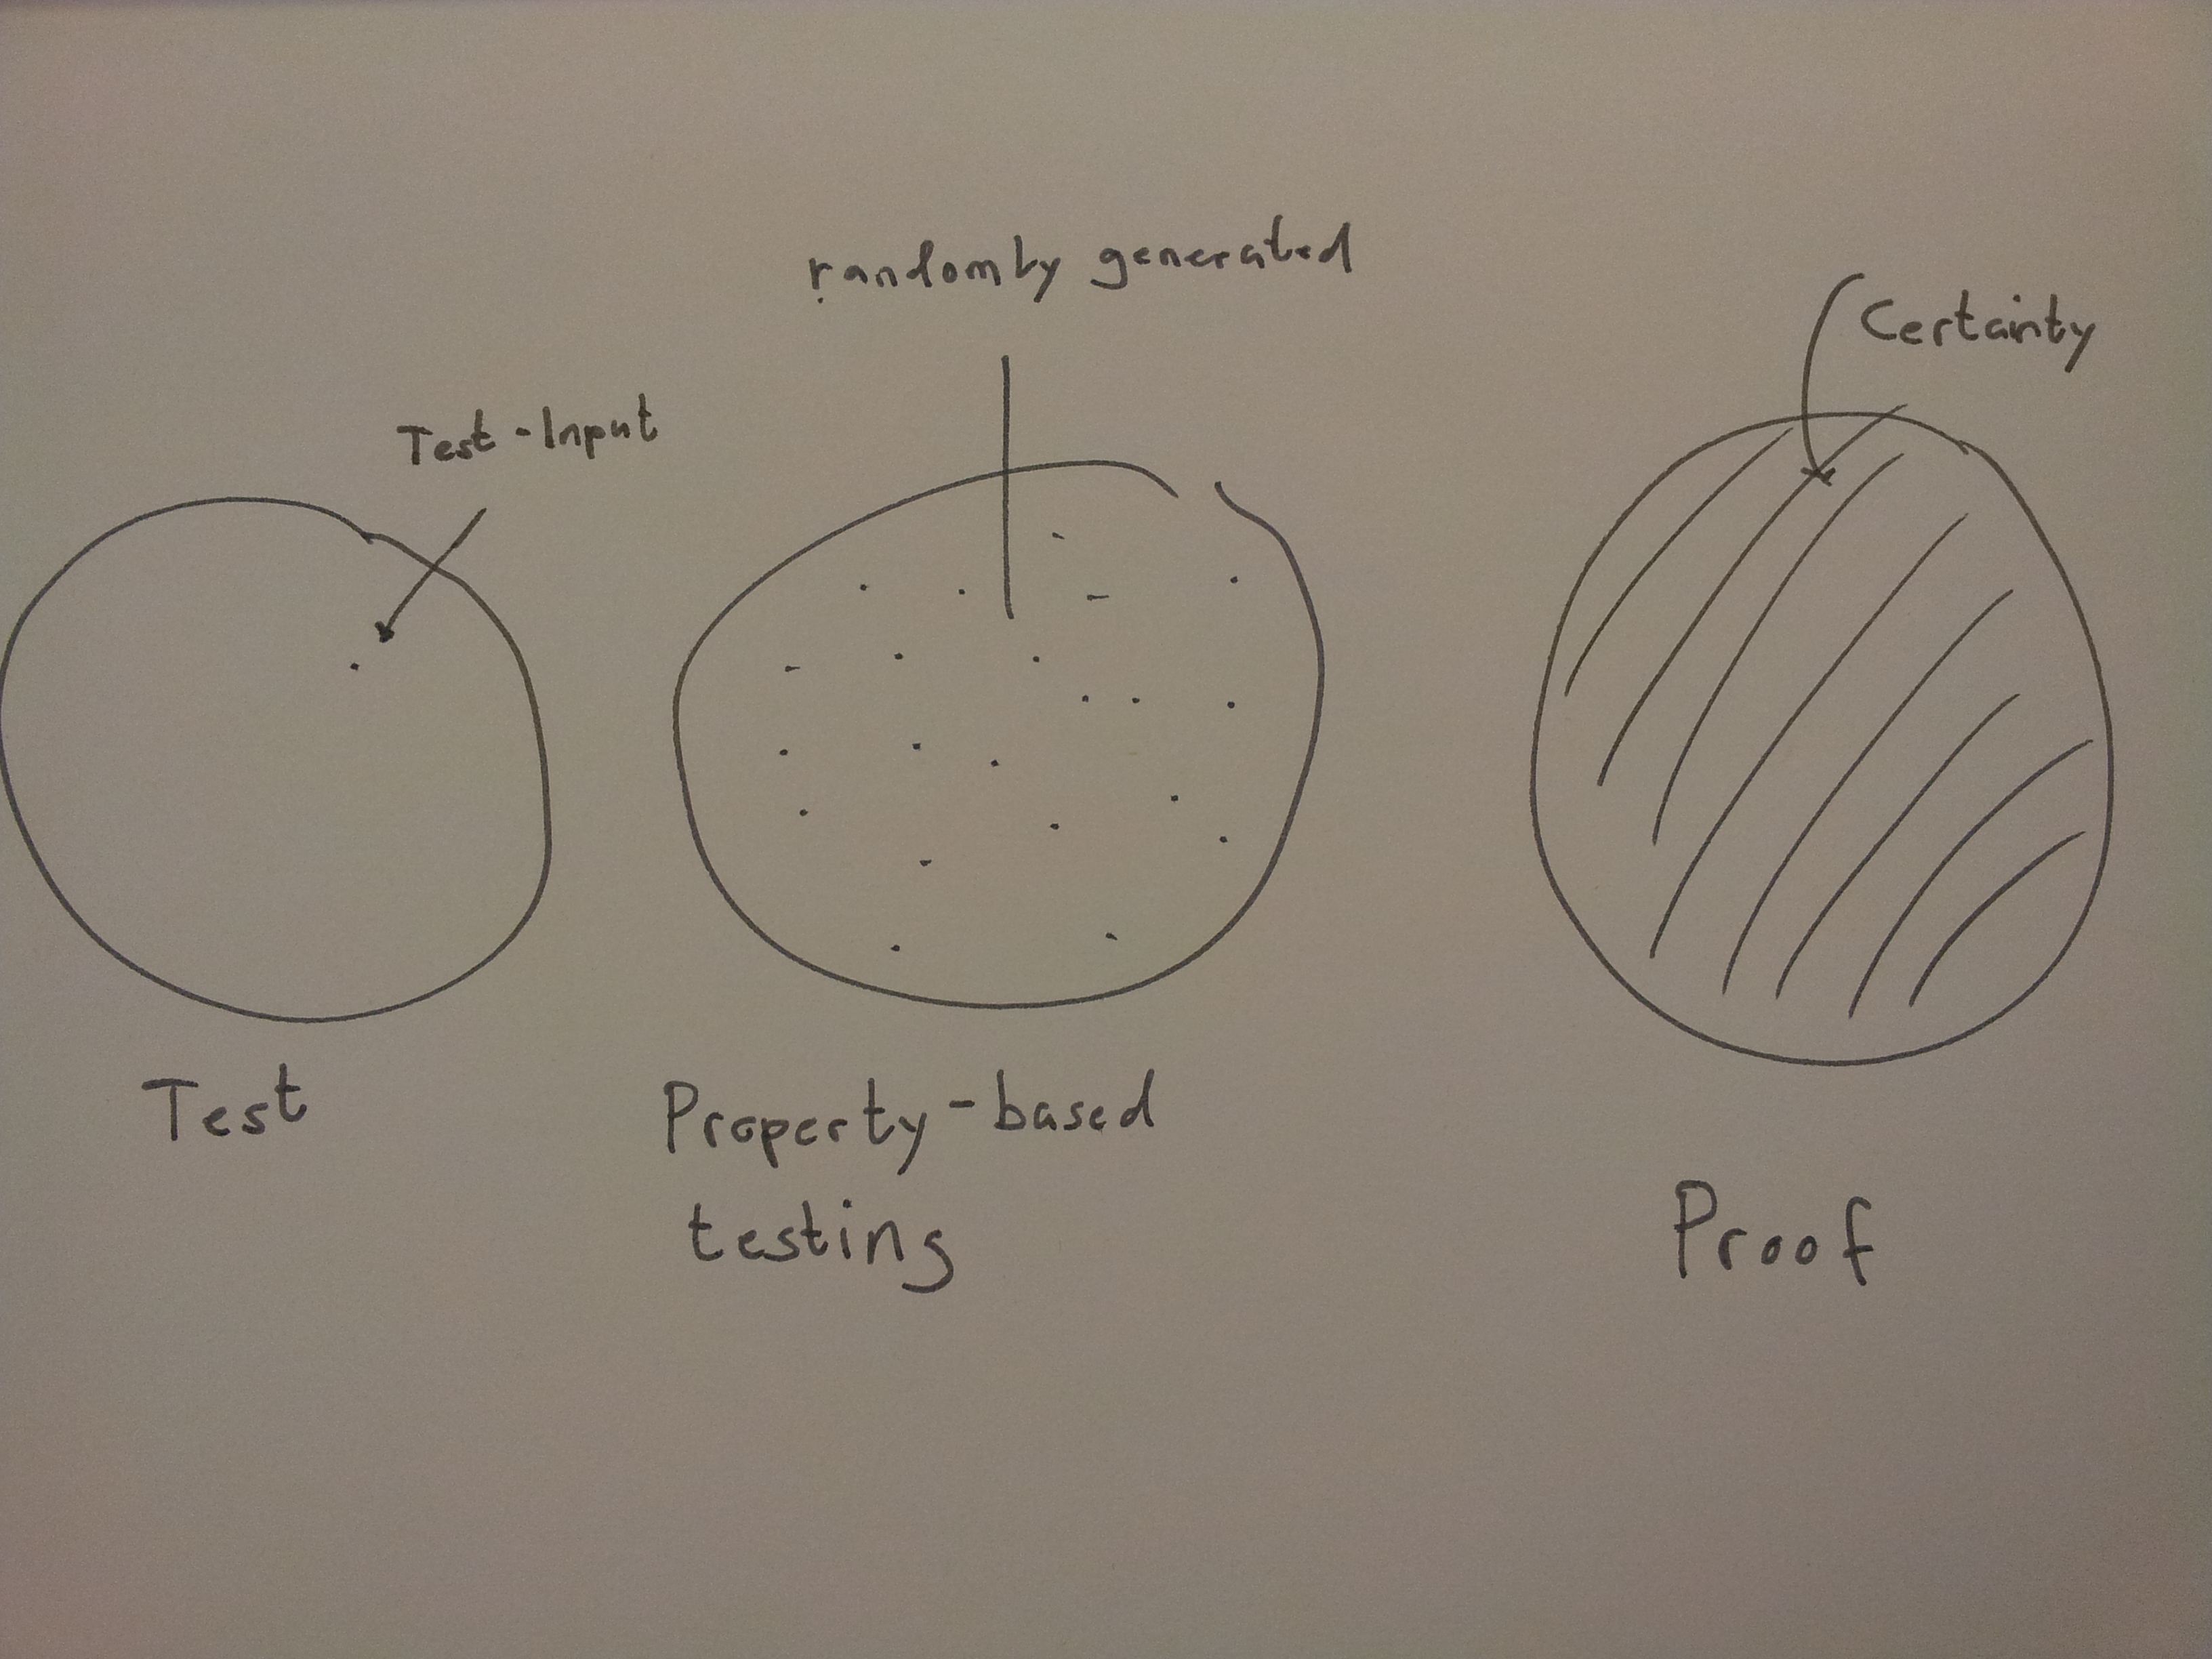
\includegraphics[width=0.9\textwidth]{comp}
  \caption{Comparison of test, property-based-testing and proof}
  \label{fig:property_validation}
\end{figure}

Equational reasoning isn't a method only used in programming. Equational reasoning is the process of substituting expressions. With equational reasoning we are able to show that certain properties hold.
For example, it's possible to show that

\begin{equation}
  \label{eq:sum}
  (x+a)(x+b) = x^2 + (a+b)x+ab
\end{equation}

is true. To show the equality we have to only have to substitute the expression on the left-hand side with the help of the basic algebraic properties of numbers (commutative, associative, distributive) \cite{hutton}.

A function definition in Haskell means that we can substitute the lefthand side. Hence, we can use reasoning about a Haskell program in the same way, we reason about mathematical expressions. With equational reasoning it's possible to deduce properties from definitions.

For example, it's possible to show that 
\begin{verbatim}
length [x] == 1
\end{verbatim}
no matter what \verb|x| is.

This article will only describe proofs with programs, which halts. An evaluation can go on forever.
\begin{verbatim}
f x = 1 + f x
\end{verbatim}

The value of the expression is undefined. The proofs in this article hold only for defined expressions and finite lists..

Equational reasoning is usefull because
\begin{itemize}
\item it allows to verify propererties of a program.
\item can be used to eliminate expensive function call while preserving behavior
\end{itemize}

\subsection{Proof by structural induction}
\label{sec:induction}

The technique proof by induction is often used to reason about programs that involve recursion. The principle of induction states that it is sufficient to prove a property $p$ for the base case and that $p$ is preserved by the inductive case.

Proof by induction is similar to write a recursive function. Recursive functions use a base case (e.g. \verb|[]|, 0). 
If we use structural induction we proof the base case.

A recursive function definition we define \verb|f (x:xs)| and use \verb|f x| in the right-hand side. In the proof we show that $p(n+1)$ with the assumption $p(n)$.

The pattern for structural induction for proofing a property can be use for list or algeraic data types with a recursice constructor (e.g. Tree).

We use induction to prove the following property
\begin{equation}
  \label{eq:lengthprop}
  \text{length (xs ++ ys)} = \text{(length xs) ++ (length ys)}
\end{equation}

The Prelude functions \verb|length| and \verb|(++)| are defined as follows:
\begin{program}
\begin{verbatim}
length [] = 0
length (x:xs) = 1 + length 
\end{verbatim}
\caption{Definition length function}
\label{lst:lengthdefinition}  
\end{program}

\begin{program}
\begin{verbatim}
[] ++ xs = xs
(x:xs) ++ ys = x:(xs++ys)
\end{verbatim}
\caption{Definition: ++ - function}
\label{lst:catdefinition}  
\end{program}

First we have to show that property \ref{eq:lengthprop} holds for the base case. The base case, in this example, are the arguments \verb|[]| and a arbritrary list for \verb|ys|. It isn't necessary to replace \verb|ys| because, the definition of \verb|++| uses recursion over \verb|xs|. \verb|ys| will always be the same list.
In order to check if property \ref{eq:lengthprop} holds for the base case, we replace \verb|xs| with  \verb|[]|, leading to

\begin{program}
\begin{verbatim}
length ([] ++ ys) = length [] + length ys
\end{verbatim}
\caption{Base case}
\label{lst:equality1}
\end{program}

We will evaluate the expression on the left-hand side and the right and side separately.

The left-hand side evaluates to
\begin{program}
\begin{verbatim}
length ([] ++ ys) -- apply ++
length ys
\end{verbatim}
\end{program}

The right-hand side evaluates to 
\begin{program}
\begin{verbatim}
length [] + length ys     -- apply length []
0 + length ys
length ys
\end{verbatim}
\end{program}

Both sides of the function definition in Listing \ref{lst:equality1} are equal. Hence, property \ref{eq:lengthprop} holds for the empty list, our base case.

Now we have to prove the induction step. We have to prove that
\begin{equation}
  \label{eq:induction}
    \text{length ((x:xs) ++ ys)} = \text{(length (x:xs)) ++ (length ys)}
\end{equation}

with the assumption (induction hypothesis)
\begin{equation}
  \label{eq:induction_hypothesis}
      \text{length (xs ++ ys)} = \text{(length xs) ++ (length ys)}
\end{equation}

Again, we evaluate the the left hand side of equation \ref{eq:induction}.

\begin{program}
\begin{verbatim}
length ((x:xs) ++ ys)}     --apply definition of ++
length (x:(xs ++ ys))      --apply definition of length
1 + length (xs ++ ys)      --use induction hypothesis
1 + length xs + length ys
\end{verbatim}
\end{program}

If we evaluate the right-hand side of the induction step in equation  \ref{eq:induction} we get:
\begin{program}
\begin{verbatim}
length (x:xs) + length ys    -- apply definition of length
1 + length xs + length ys
\end{verbatim}
\end{program}

The last listing shows, that the equation \ref{eq:induction} follows from the induction hypothesis in equation \ref{eq:induction_hypothesis}. This completes the induction step and therefore the proof itself.

\section{Pipes}
\label{sec:pipes}

Pipes is a streaming library for Haskell. It was build with the following requirements \cite{gonzales13}.
\begin{description}
\item[Effects] Streams has to be effectful
\item[Streaming] Processing in constant memory
\item[Composability] Modules have to be composable
\end{description}

Pipes uses the type class \verb|Category| too keep the API simple and easy to use.

This article will descipe a part of the library with an example.

First we need a input stream, that emits values. Input streams are have the type 
\verb|Producer a m ()|.
Listing \ref{lst:simpleproducer} show a simple Producer. It emits the integers 1,2 and 3. It is also possible to create producers for effectful streams. We use the simple producer from Listing \ref{lst:simpleproducer} for simplicity reasons.

\begin{program}
\begin{verbatim}
produceints123 :: Producer Int IO ()
produceints123 = each [1,2,3]
\end{verbatim}
\caption{Simple Producer}
\label{lst:simpleproducer}
\end{program}

Pipes provide the function \verb|for| to consume a producer. 
\verb|for producer body| loops over the \verb|producer| and applies a the transformation defined in \verb|body| to every element yielded by the producer. If the body is of type \verb|Effect| it return an \verb|Effect|. If body is of type \verb|Producer| a \verb|Producer| is returned. The type declaration of \verb|for| is
\begin{program}
\begin{verbatim}
for::Monad m=>Producer b m r->(b -> Producer c m ())->Producer c m r
\end{verbatim}
\caption{type of for}
\end{program}

If we apply \verb|for| we get another producer. This means are able to compose several Producers.

\section{Function composition}

\label{sec:functioncomposition}

Function composition in mathematics is defined as

\begin{equation}
  \label{eq:functioncomposition}
  (f \circ g)(x) = f(g(x))
\end{equation}

Haskell functions can be compose with the \verb|.| function.

\begin{figure}
  \centering
\begin{verbatim}
(.) :: (b -> c) -> (a -> b) -> a -> c
f . g = \x -> f (g x)
\end{verbatim}
  \caption{. function}
  \label{fig:compositionfunction}
\end{figure}

Function composition allows us to create a function by composing it with many small functions. 

Functions in Haskell form a category in category theory. They satisfy the category laws.
\begin{description}
\item[Associativity law] 
\item[Left/Right Identity law] 
\end{description}

\bibliographystyle{plain}
\bibliography{a}
\end{document}